\chapter{Zagotavljanje varnosti v sodelovalni aplikaciji z robotom Motoman HC10DT}%

\begin{mdframed}[backgroundcolor=green!20, shadow=true,roundcorner=8pt]
	\vspace{-0.35cm}
	
	\section{Cilj vaje}
	
	Pri tej vaji boste spoznali različne varnostne funkcije, ki se jih lahko implementira v konceptu sodelovalne aplikacije. Varnostne elemente boste uporabili v povezavi s sodelujočim robotom Motoman HC10DT proizvajalca Yaskawa. V prvem delu vaje boste definirali parametre in varnostno ovojnico prijemala in objekta v delovnem prostoru robota, nato pa testirali delovanje preprečevanja trka med robotom in objektom. V drugem delu vaje boste implementirali varnostni način nadzora sile in moči na tak način, da se bo robot ob trku z operaterjem  odmaknil ter s tem preprečil poškodbo operaterja. Tretji del zajema uporabo laserskega skenerja proizvajalca SICK za definiranje treh varnostnih območij. Na podlagi informacije o lokaciji uporabnika boste ustrezno prilagodili hitrost gibanja robota.
	
\end{mdframed}

\section{Sodelovanje človek--robot}

Sodelovanje med človekom in robotom združuje lastnosti obeh akterjev: človeško inteligenco, prilagodljivost in sposobnost rokovanja z nedeterminiranimi materiali ter robotsko vzdržljivost, natančnost in moč. Pri tem je neizogibno, da človek in robot opravljata nalogo v neposredni bližini. Tehnično priporočilo standardu ISO/TS 15066:2016 predpisuje zahteve za različne načine sodelovanja. Pomembna je tudi ocena tveganja celotnega sistema (ta vključuje robota, prijemalo, obdelovanec, periferijo, človeka), s katero identificiramo potencialno nevarne situacije ter rešitve, kako se jim izogniti.

Skupno delovanje človeka in robota lahko razdelimo na tri dele:
\begin{itemize}
	\item \textbf{soobstoj} -- robot in delavec sta prisotna v skupnem prostoru, robot je ločen od delavca, ne more priti do kontakta med robotom in delavcem,
	\item \textbf{kooperacija} -- robot in delavec si delita delovni prostor, naloge izvajata simultano na ločenih objektih, interakcija z robotom prek skupnega delovnega prostora, kjer si izmenjujeta delovne objekte,
	\item  \textbf{sodelovanje} -- robot in delavec si delita delovni prostor, nalogo izvajata na simultano na skupnem objektu.
\end{itemize}


\begin{figure}[!hbt]
	\centering
	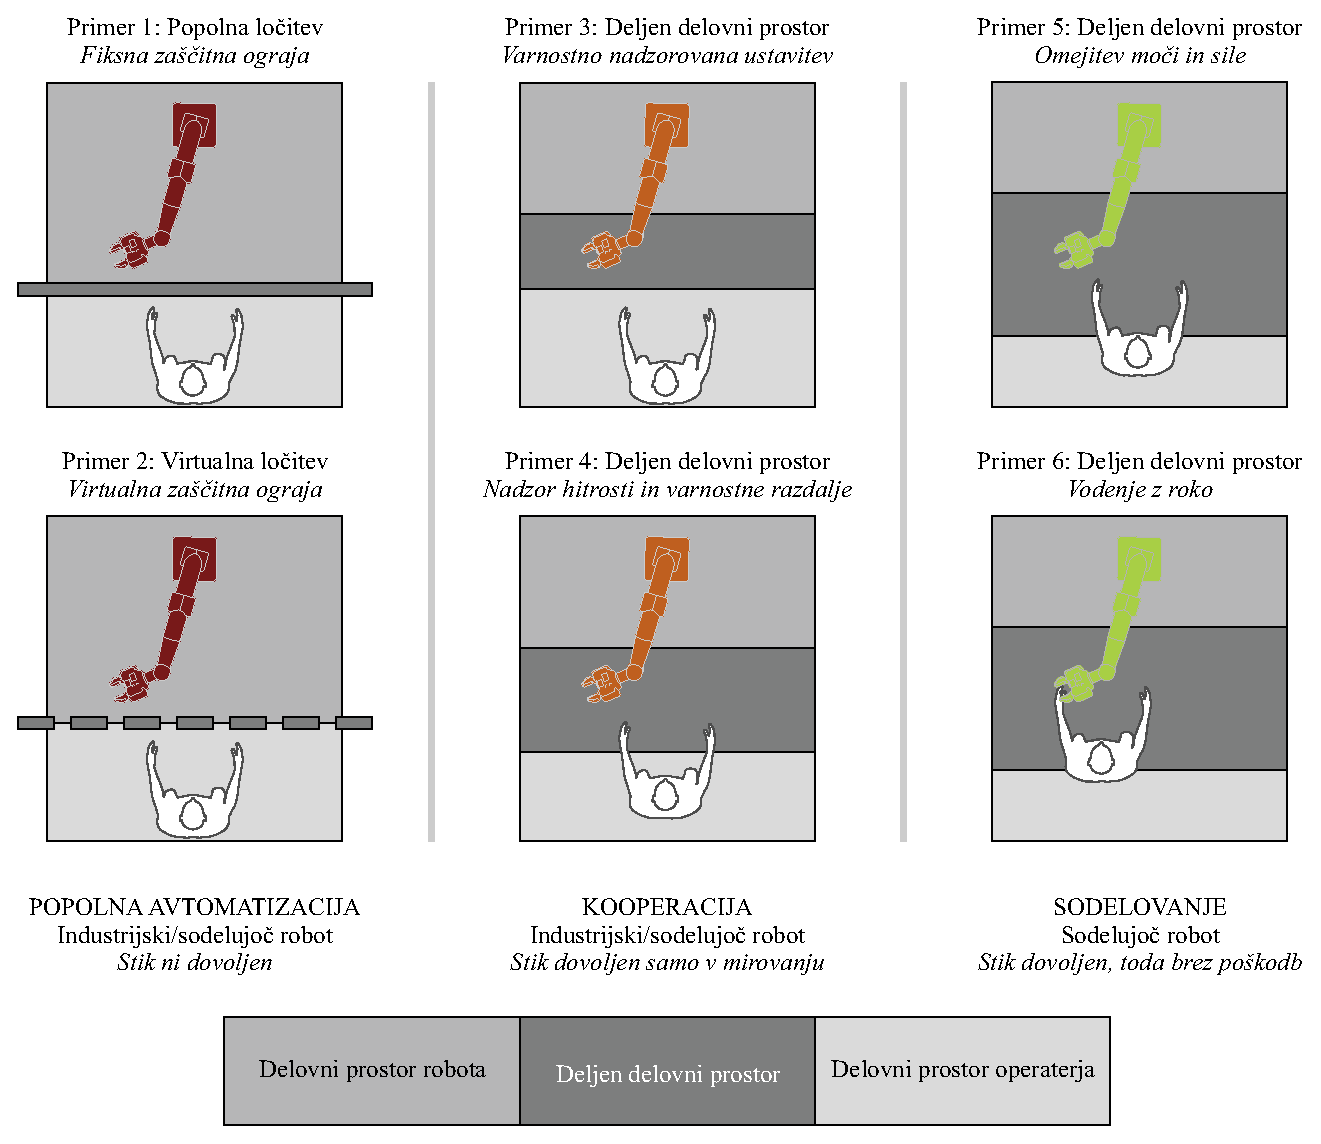
\includegraphics[width=\textwidth]{hc10_sodelovanje.eps}
	\caption{Primeri različnih načinov sodelovanja človeka in robota}
	\label{fig:hc10_sodel}
\end{figure}


Za zagotavljanje varnosti operaterja mora imeti robot implementirano vsaj eno izmed štirih kategorij varnosti:
\begin{itemize}
	\item \textbf{varnostno nadzorovana ustavitev} -- v primeru nevarne situacije se robot ustavi (motorji so prižgani),
	\item \textbf{vodenje z roko}  -- operater lahko ročno vodi robota, enostavnejše programiranje in izvajanje aplikacij,
	\item \textbf{nadzor hitrosti in varnostne razdalje} -- hitrost robota se prilagaja glede na oddaljenost človeka od robota (različne cone hitrosti, bližje kot je operater robotu, manjša je hitrost), potrebni dodatni senzorji (laserski skenerji, svetlobne zavese, ...)
	\item \textbf{omejitev moči in sile} -- robot deluje z ustrezno močjo, da v primeru nehotenega trka z operaterjem ne pride do poškodbe, ISO/TS 15066:2016 podaja ustrezne sile/pritiske za posamezna področja človeškega telesa, kompromis med hitrostjo in nosilnostjo robota.
\end{itemize}


\section{Struktura sistema}

Robotski sistem sestavlja sodelujoči robot Yaskawa Motoman HC10DT s krmilnikom YRC1000, robotsko prijemalo OnRobot RG2 ter laserski skener SICK TIM310-1130000. Celotna konfiguracija je predstavljena na sliki \ref{fig:hc10_sistem}.

\begin{figure}[!hbt]
	\centering
	\includegraphics[width=0.9\textwidth]{hc10_sistem.eps}
	\caption{Robotski sistem}
	\label{fig:hc10_sistem}
\end{figure}

\subsection{Motoman HC10DT}

Robot je predstavnik sodelujočih robotov, ki so narejeni za varno delo skupaj s človekom brez dodatnih varnostnih elementov (varnostnih ograj, svetlobnih zaves ...), seveda v skladu z analizo tveganja. Robotska roka je antropomorfne oblike s 6 prostostnimi stopnjami. Posamezni sklep robota je opremljen s senzorjem navora, ki na nivoju sklepa meri interakcijo robota z okolico. Robota se lahko premika z roko, za shranjevanje ukazov pa se lahko uporablja vmesnik na vrhu robota, kar omogoča prihranek časa pri programiranju robota.

Osnovni podatki robotske roke so podani v tabeli \ref{tab:hc10}.

\begin{table}
	\centering
	\caption{Specifikacije robota Yaskawa Motoman HC10DT} \label{tab:hc10}
	\begin{tabular}{|lr|c|}
		\hline   Tip &  & HC10DT \\
		\hline Doseg & & $1,2$ m \\
		\hline Nosilnost  & & $9$ kg \\
		\hline Hitrost vrha& & $1$ m/s \\
		\hline Hitrost vrha (varen način)& & $0,25$ m/s \\
		\hline Ponovljivost pozicioniranja& & $\pm 0.1$ mm \\
		\hline Maksimalna hitrost
		& Os 1 & $130$ $^\circ/s$ \\
		& Os 2 & $130$ $^\circ/s$ \\
		& Os 3 & $180$ $^\circ/s$ \\
		& Os 4 & $180$ $^\circ/s$ \\
		& Os 5 & $250$ $^\circ/s$ \\
		& Os 6 & $250$ $^\circ/s$ \\
		\hline Delovni prostor
		& Os 1 & $\pm180^\circ$\\
		& Os 2 & $\pm180^\circ$\\
		& Os 3 & $-5^\circ/+355^\circ$\\
		& Os 4 & $\pm180^\circ$\\
		& Os 5 & $\pm180^\circ$\\
		& Os 6 & $\pm180^\circ$\\
		\hline   Teža &  & $48$ kg \\
		\hline
	\end{tabular}
\end{table}

Robot lahko deluje v dveh načinih. Prvi je kot klasični industrijski manipulator, kjer je maksimalna hitrost vrha deklarirana na 1000~mm/s. V tem načinu je potrebno robota ločiti od delavcev z varnostnimi elementi (ograje, svetlovne zavese). Drugi način pa je kot sodelujoči robot. V tem načinu je hitrost vrha omejena na 250~mm/s. Pri tej hitrosti in deklarirani nosilnosti robot v primeru trka s človekom ne povzroči poškodbe (glede na specifikacije ISO/TS 15066:2016).

Robota se programira z uporabo ročne učne enote (slika \ref{fig:hc10_pendant}). Ta omogoča premikanje robota, upravljanje s prijemali, pisanje, popravljanje in poganjanje programov ter podobno.

\begin{figure}[!hbt]
	\centering
	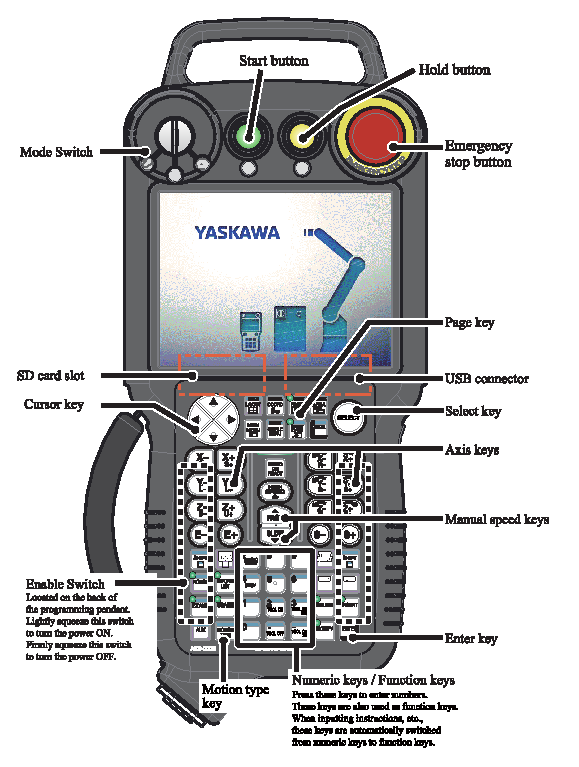
\includegraphics[width=0.9\textwidth]{hc10_pendant.eps}
	\caption{Ročna učna enota}
	\label{fig:hc10_pendant}
\end{figure}

Robot HC10DT je opremljen z integriranim varnostnim krmilnikom FSU (Functional Safety Unit), ki omogoča različne varnostne funkcije. S FSU se lahko nastavi dovoljena območja gibanja posameznega sklepa, maksimalne dovoljene hitrosti za posamezni sklep ter za vrh robota, ter se definira različna območja delovanja (območje, ki ga robot ne sme zapustiti, območje, v katerega robot ne sme vstopiti, ravnine, ki omejujejo gibanje robota).

\subsection{Prijemalo OnRobot RG2}

Prijemalo OnRobot RG2 spada v kategorijo sodelujočih prijemal. Prijemalo omogoča pozicijsko vodenje in vodenje po sili, obenem pa ima integrirano detekcijo stanja prijemanja (objekt prijet/spuščen, prijemanje, širina prijetega objekta). Konfiguracija prstov omogoča tako zunanje kot tudi notranje prijemanje objektov. Specifikacije prijemala so podane v tabeli \ref{tab:RG2}, dimenzije pa so predstavljene na sliki \ref{fig:hc10_onrobot}.

\begin{table}
	\centering
	\caption{Specifikacije prijemala OnRobot RG2}
	\label{tab:RG2}
	\begin{tabular}{|l|c|}
		\hline Tip                  & OnRobot RG2 \\
		\hline Premik prstov        & $0-110$ mm \\
		\hline Ponovljivost prstov   & $\pm 0,1$ mm \\
		\hline Sila prijemanja      & $3-40$ N \\
		\hline Ponovljivost sile    & $\pm 1$ N \\
		\hline Teža                 & $0,65$ kg \\
		\hline
	\end{tabular}
\end{table}


\begin{figure}[!hbt]
	\centering
	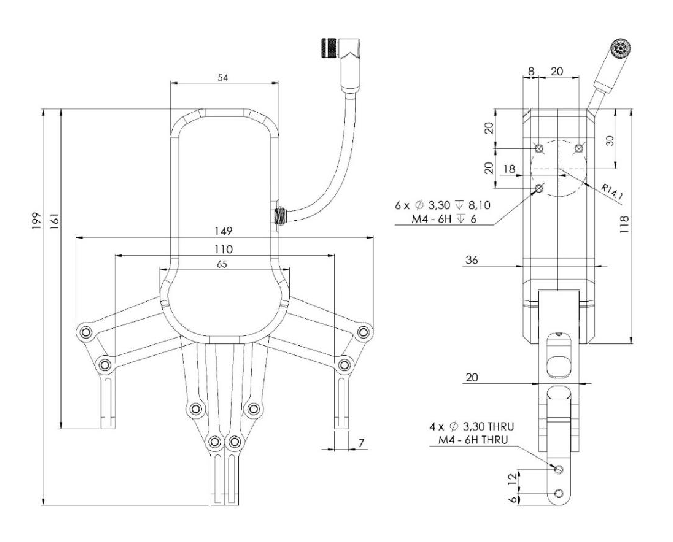
\includegraphics[width=0.9\textwidth]{hc10_onrobot.eps}
	\caption{Dimenzije prijemala OnRobot RG2}
	\label{fig:hc10_onrobot}
\end{figure}


\subsection{Laserski skener SICK TIM310}

Laserski skener SICK TIM310 detektira objekte v različnih področjih glede na odboj laserskega žarka. Doseg skeniranje je do 4~m. Senzor podpira nastavitev treh delno prekrivajočih področij enake oblike vendar različnih velikosti (glej sliko \ref{fig:hc10_sick}). Oblike področij so  v naprej definirane ali pa jih uporabnik nastavi sam. Senzor sporoča v katerem polju se nahaja objekt preko digitalnih linij (vsako področje ima ločeno linijo), zato je z robotskim krmilnikom (FSU) povezan preko digitalnih vhodov.

\begin{figure}[!hbt]
	\centering
	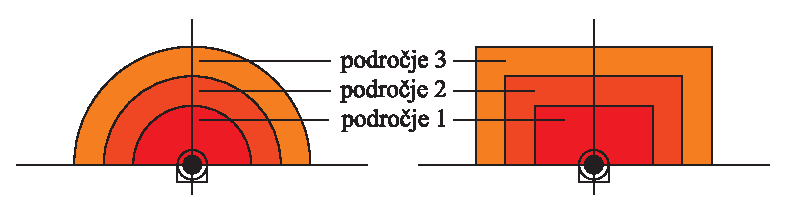
\includegraphics[width=0.9\textwidth]{hc10_podrocja.eps}
	\caption{Primera polkrožnega in pravokotnega področja zaznavanja senzorja}
	\label{fig:hc10_sick}
\end{figure}

Za nastavljanje področij in parametrov senzorja se uporablja program SOPAS. Ta omogoča nastavljanje oblike in velikosti področij, odzivni čas zaznave posameznega področja, velikost objektov, ki jih zanemari, in čas signaliziranja o detektiranem objektu.

\section{I. del: Definiranje orodja in objektov}

\subsection{Izvedba na realnem robotu}

Na prirobnico robota je nameščeno prijemalo OnRobot RG2. S pravilno definicijo orodja robotski krmilnik upošteva dimenzije in parametre orodja za ustrezno izvajanje programa in nalog. Za definicijo orodja odprite meni \textbf{TOOL}, ki se nahaja v meniju \textbf{ROBOT}, kot je prikazano na sliki \ref{fig:hc10_tool1}.

\begin{figure}[!hbt]
	\centering
	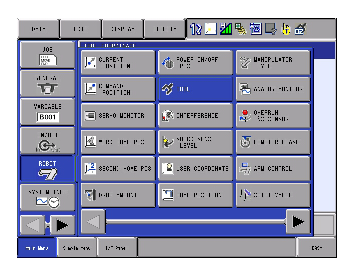
\includegraphics[width=0.7\textwidth]{hc10_tool1.eps}
	\caption{Meni TOOL}
	\label{fig:hc10_tool1}
\end{figure}

\subsection*{Kalibracija orodja}

V meniju \textbf{TOOL} se nahaja seznam definiranih orodij. S smernimi tipkami se postavite na orodje številka 5 (\verb"OnRobot_VS") nato pa ga izberite s tipko \textbf{SELECT}. Odpre se vam novo okno \textbf{TOOL}, kjer so zapisani določeni parametri prijemala. V področju izbire menijev izberete opcijo \textbf{UTILITY} in nato iz zavesnega menija še \textbf{CALIBRATION}. V področju izbire menijev izberete opcijo \textbf{DATA} in nato še \textbf{CLEARDATA}, da zbrišete prejšnje podatke. Odločitev je potrebno potrditi s pritiskom gumba \textbf{YES}, ki se pojavi na zaslonu.

\begin{itemize}
	\item V robotsko prijemalo vpnite kalibracijsko konico. V meniju \textbf{IN/OUT > GENERAL PURPOSE OUTPUT} se nahaja seznam vhodno/izhodnih linij robota. Prijemalo OnRobot je povezano na izhodno linijo \verb"OUT#0015". S klikom na \textbf{Page} odprete okno \textbf{Group\_no.} in vpišete \textbf{2}, da se premaknete na seznam izhodov od 9 do 16. Nato se premaknete na krožec pred imenom, kjer s kombinacijo tipk \textbf{INTERLOCK + SELECT} vklapljate in izklapljate izhod in s tem odpirate in zapirate prijemalo.
	\item S prijemalom se premaknite do kalibracijske konice na mizi (konici približate).
	\item Nato izberete kalibracijsko točko \textbf{TC1}, ter pritisnete tipki \textbf{MODIFY} in nato še \textbf{ENTER}. Pri tem morajo biti motorji robota prižgani.
	\item Nato premaknite robota v drugo orientacijo, kjer se konici stikata, izberite točko \textbf{TC2}, ter \textbf{MODIFY} in \textbf{ENTER}.
	\item Postopek ponovite še za ostale tri točke \textbf{TC3}, \textbf{TC4} in \textbf{TC5}. Pri tem pazite, da so orientacije orodja čim bolj različne.
	\item Ko zaključite učenje kalibracijskih točk za kalibracijo novega vrha robota, pritisnete tipko \textbf{COMPLETE}. Tako se avtomatsko izračuna lega novega orodja glede na lego zadnjega segmenta robota.
\end{itemize}

S tem postopkom ste določili geometrijo orodja, potrebno pa je nastaviti še maso in položaj težišča orodja. To storite tako, da se s smernimi tipkami postavite na ustrezno polje, s tipko \textbf{SELECT} polje izberete ter vpišete ustrezno vrednost. Ko vpišete vse parametre, je potrebno definicijo shraniti. Najprej izberete gumb \textbf{READBACK}, nato pa \textbf{WRITE}. Odpre se okno \textbf{Update the file?}, izberete \textbf{YES}.

Parametri prijemala so podani v tabeli  \ref{tab:rg3}.
\begin{table}
	\centering
	\caption{Parametri prijemala OnRobot RG2} \label{tab:rg3}
	\begin{tabular}{|l|c|}
		\hline W    & $1,525$ kg \\
		\hline Xg   & $-76,450$ mm \\
		\hline Yg   & $-53,300$ mm \\
		\hline Zg   & $50,250$ mm \\
		\hline
	\end{tabular}
\end{table}

\subsection*{Preverjanje kvalitete kalibracije orodja}

Robota postavite prosto v prostor. S tipko \textbf{COORD} izberete premikanje robota v koordinatnem sistemu orodja. Spreminjanje koordinatnih
sistemov spremljate v statusni vrstici. Deklarirano orodje morate nato izbrati s pomočjo učne enote s tipkama\textbf{ SHIFT + TOOL SEL}. Izbrano orodje je prikazano v menijski vrstici na vrhu zaslona (glej sliko \ref{fig:hc10_tool3}).

\begin{figure}[!hbt]
	\centering
	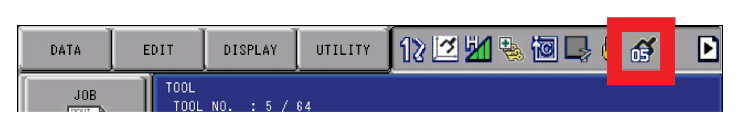
\includegraphics[width=0.7\textwidth]{hc10_tool3.eps}
	\caption{Izbrano orodje}
	\label{fig:hc10_tool3}
\end{figure}

Kvaliteto kalibracije preverite z rotacijami (tipke na desni strani učne enote) orodja okrog koordinatnih osi izbranega koordinatnega sistema orodja. če konica kazalnika pri tem v prostoru navidezno miruje, je kvaliteta kalibracije konice zadovoljiva, drugače postopek ponovite.

\subsection*{Varnostna ovojnica prijemala}

Po deklaraciji je potrebno orodju določiti še parametre varnostne ovojnice valjev za detekcijo trkov z navideznimi varnostnimi območji. Izbranemu orodju določimo parametre ovojnic z menijem \textbf{ROBOT > TOOL INTERFERE}. Okoli orodja je mogoče določiti pet različnih ovojnic v obliki valjev. Primer varnostne ovojnice za prijemalo RG2 (dva valja) je prikazan na sliki \ref{fig:hc10_ovoj1}.

\begin{figure}[!hbt]
	\centering
	\includegraphics[width=\textwidth]{hc10_ovoj1.eps}
	\caption{Prikaz ovojnic (valjev) okoli orodja za prijemalo OnRobot RG2. Označen koordinatni sistem predstavlja koordinatni sistem vrha robota.}
	\label{fig:hc10_ovoj1}
\end{figure}

Preden začnete vpisovati parametre, preverite, da vpisujete parametre za pravo orodje (\textbf{TOOL NO.}). Na sliki \ref{fig:hc10_ovoj2} je izbrano orodje prikazano v zgornjem rdečem okviru). Pravilno orodje izberete z izbiro gumba \textbf{PAGE}. Vsaki ovojnici določite točko na skrajnih legah in radij valja. Pri tem si pomagajte s sliko \ref{fig:hc10_ovoj1}. Skrajne lege ovojnic morate definirati glede na koordinatni sistem vrha robota. Ko vpišete parametre, ne pozabite parametrov shraniti z \textbf{READBACK > WRITE > YES}. V meniju \textbf{SAFETY FUNC. > OPERATION AREA MONITOR} si lahko ogledate grafični prikaz ovojnic, ki ste jih vpisali. če katerikoli valj, ki ste ga določili, vstopi v varnostno področje, FSU sistem javi, da je prišlo do dotika z varnostnim področjem.

\begin{figure}[!hbt]
	\centering
	\includegraphics[width=0.7\textwidth]{hc10_ovoj2.eps}
	\caption{Parametri ovojnic za prijemalo OnRobot. Bodite pazljivi, da imate izbrano pravo orodje (zgornji rdeč okvir)}
	\label{fig:hc10_ovoj2}
\end{figure}

\subsection*{Definiranje varnostnega območja}

V nadaljevanju preizkusite varnostni mehanizem uporabe navideznih varnostnih območij. Na mizo postavite škatlo (pravokotno na koordinatni sistem baze), ki vam bo služila kot fizični model varnostnega območja. V meniju \textbf{SAFETY FUNC. > ROBOT RANGE LIMIT} boste vpisali podatke za varnostno območje v obliki kvadra. Primer parametrov je podan na sliki \ref{fig:hc10_ovoj3}
\begin{itemize}
	\item V polju \textbf{FILE NO.} je vpisana zaporedna številka polja.
	\item V polje \textbf{COMMENT} vpišete ime območja.
	\item V polju \textbf{ALARM} izberete možnost \textbf{ON(MOVE STOP)}. S tem izberete možnost, da se robot ustavi, ko vstopi v varnostno območje.
	\item V polju \textbf{MONITOR TARGET} izberete možnost \textbf{OUTSIDE}.
	\item V polju \textbf{SHAPE TYPE} izberete možnost \textbf{CUBOID} (oblika varnostnega območja bo kvader). Mere kvadra bodo določene z dvema skrajnima, diagonalno nasprotnima,  ogliščema, ki jih vpišete v polji  \textbf{POINT1} in \textbf{POINT2}. Ti dve točki sta podani glede na bazni koordinatni sistem robota. Točki bi lahko odmerili ročno z merilnim trakom, vendar raje uporabite vrh robota. Prijemalo postavite v ustrezno ogljišče, pri čemer upoštevajte, da mora biti ovojnica kakšen cm večja od dimenzij objekta, da zagotovite, da se robot ustavi še predno pride do fizičnega kontakta. V meniju \textbf{ROBOT > CURRENT POSITION} nastavite \textbf{COORDINATE} na bazni koordinatni sistem \textbf{BASE} (tipka \textbf{SELECT}). Preverite, da je izbrano orodje št. \verb"TOOL:05". Vrednosti, ki so zapisane pod \verb"R1:X, Y, Z" predstavljajo koordinate oglišča varnostnega območja in jih vpišete v polje \textbf{POINT1}. Nato robota prestavite v drugo oglišče ter ponovite postopek še za točko \textbf{POINT2}.
\end{itemize}

\begin{figure}[!hbt]
	\centering
	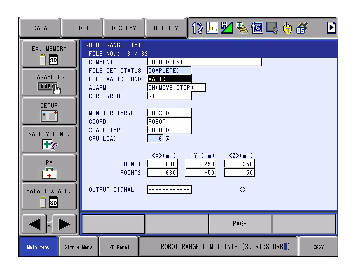
\includegraphics[width=0.7\textwidth]{hc10_ovoj3.eps}
	\caption{Parametri varnostnega področja}
	\label{fig:hc10_ovoj3}
\end{figure}

Na zadnje v polju \textbf{FILE VALID COND} izberete možnost \textbf{VALID}. S tem potrdite, da bo FSU enota preverjala trk med navideznim varnostnim področjem in ovojnicami robota z orodjem. Na seznamu varnostnih področij imate lahko namreč vpisanih več različnih področij, ki jih nato po potrebi vklapljate in izklapljate  v polju \textbf{FILE VALID COND}. Možnost \textbf{VALID} pomeni, da se bo trk preverjal, možnost \textbf{INVALID} pa pomeni, da FSU ne upošteva varnostnega področja pri analizi trka.

\subsection*{Test preprečevanja trka med objekti}

Z menijem \textbf{SAFETY FUNC. > OPERATION AREA MONITOR} izberete vizualni prikaz varnostnih področij in ovojnic robota. V oknu \textbf{Operation Area Monitor} najprej v polju \textbf{File No:} izberete številko vašega varnostnega področja. Z gumbi \textbf{Change Plane} izbirate pogled na robota in  varnostno območje. Premaknite robota tako, da ni v stiku z varnostnim območjem (recimo nad varnostno območje). Robota nato pomaknite navzdol, da bo prispel v stik z varnostnim področjem. Ko pride do trka, se v oknu \textbf{Operation Area Monitor} ovojnica, ki pride v stik z varnostnim področjem obarva z rdečo, kot je to prikazano na sliki \ref{fig:hc10_ovoj4}.

\begin{figure}[!hbt]
	\centering
	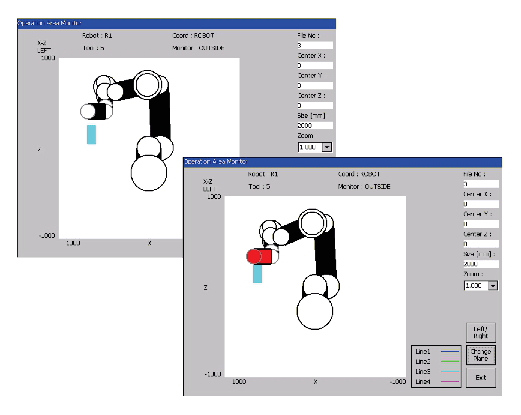
\includegraphics[width=0.9\textwidth]{hc10_ovoj4.eps}
	\caption{Prikaz trka med ovojnicami robota in orodja ter varnostnega področja (moder pravokotnik)}
	\label{fig:hc10_ovoj4}
\end{figure}

V nadaljevanju ustvarite nov robotski program (\textbf{JOB > CREATE NEW JOB}). V polju \textbf{JOB NAME (***)} pritisnete tipko \textbf{SELECT} in odprete okno za
definiranje imena programa. Za potrditev imena pritisnete tipko \textbf{ENTER}. Parametre novega programa potrdite s tipko \textbf{EXECUTE}.

Nato postavite robota nad škatlo ter shranite to točko kot linearni gib (ukaz \verb"MOVL V=900"; če je potrebno, ga nastavite s tipko \textbf{MOTION TYPE}). Točko shranite tako, da imate prižgane motorje ter pritisnete tipko \textbf{ENTER}. Robota nato prestavite na eno stran škatle ter to točko ponovno shranite kot \verb"MOVL". Robota prestavite še na drugo stran škatle ter shranite še to točko. Na sliki \ref{fig:hc10_ovoj5} je predstavljena shema postavitve točk.

\begin{figure}[!hbt]
	\centering
	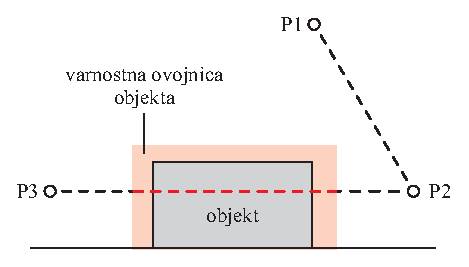
\includegraphics[width=0.6\textwidth]{hc10_ovoj5.eps}
	\caption{Primer naučenih točk za testiranje delovanja varnostnega območja. črtkana črta nakazuje predvideno pot robota.}
	\label{fig:hc10_ovoj5}
\end{figure}

Ko imate program napisan, ga je potrebno pognati v načinu \textbf{RUN}. S smernimi tipkami se postavite na začetek programa, ključ na učni enoti obrnete na srednjo pozicijo, prižgite motorje s \textbf{SERVO ON READY} ter pritisnete zeleni gumb na vrhu učne enote. Robot se mora postaviti v točko P1, nato nadaljevati pot do P2 in še naprej do P3. Ko se robot približuje škatli, se mora ustaviti še predno se zaleti v škatlo (ko vrh robota doseže rob varnostnega območja.


\section{II. del: Varnostni odmik robota} \label{poglavje2del_vaje}

Najprej izklopite ovojnico kocke, nato nadaljujte z nalogo. FSU skrbi tudi za implementacijo varnostnega protokola omejtive moči in sile. V tem primeru je kontakt med robotom in uporabnikom dovoljen, saj robot v primeru detektiranja zunanje sile aktivira varnostno nadzorovano ustavitev. Ko uporabnik potrdi, da ni več neželjenega kontakta (restart gumb na petem segmentu), robot nadaljuje z opravljanjem naloge. Zunanja sila je ocenjena na podlagi primerjave izračunanih navorov v sklepih na podlagi trenutne lege robota (in znanih dinamičnih in kinematičnih parametrih robota) ter izmerjenimi navori s sklepnimi senzorji  navora. Razlike med navori se upoštevajo kot sklepni prispevki zunanjih sil, ki delujejo na robota (kontakt).

Robot ima implementiran tudi varnostni odmik v primeru, da je sila interakcije manjša od postavljenega praga za ustavitev robota. V tem primeru ne gre za to, da se robot izogne oviri, ampak se izvede odmik v nasprotni smeri kontakta, da se prepreči poškodbe operaterja. Ko robot zazna, da ni več interakcije z okolico, se vrne v prejšnjo lego in nadaljuje z nalogo. če pa je sila večja od praga, se izvede klasična varnostno nadzorovana ustavitev.

\subsection{Izvedba naloge} \label{realni2}

Najprej z robotom definirajte pravokotnik s šestimi točkami kot je prikazano na sliki \ref{fig:hc10_move}. Za shranjevanje točk uporabite ukaz za linearni premik \verb"MOVL V=900.0".

Testirajte napisani program, da preverite, če se robot ustrezno premika po postavljenem pravokotniku. Najprej testirajte premikanje od točke do točke (gumb \textbf{FWD}), nato pa še v avtomatskem načinu (postavite se na začetek programa, ključ na ročni učni enoti obrnite na srednji pozicijo, prižgite motorje - tipka \textbf{SERVO ON READY} in poženite program z zeleno tipko na vrhu učne enote).

\begin{figure}[!hbt]
	\centering
	\includegraphics[width=\textwidth]{hc10_move.eps}
	\caption{Testni pravokotnik, sestavljen iz šestih točk (P1 -- P6). Zelena črta označuje območje, kjer je vklopljena funkcija varnostnega odmika. }
	\label{fig:hc10_move}
\end{figure}

Ko ste zadovoljni z gibanjem robota, program nadgradite tako, da je v zelenem območju (glej sliko \ref{fig:hc10_move}) aktivirana funkcija varnostnega odmika. S klicem \verb"EI LEVEL= 1" prekinitveno funkcijo vklopite, s klicem \verb"DI LEVEL= 1" pa jo izklopite. Do \verb"EI" in \verb"DI" dostopate preko tipke \textbf{INFORM LIST} in menija \textbf{Control}. Izbiro potrdite s tipko insert \textbf{ENTER}. Nato se v programu s smernimi tipkami postavite desno na \verb"EI" (oziroma \verb"DI") in izberete \textbf{Select}. Pod izbiro \textbf{INT LEVEL} spremenite \textbf{UNUSED} v \textbf{LEVEL=} ter nastavite na \textbf{1}. Nastavitev potrdite z dvema \textbf{ENTER}.

Pred zagonom nastavite še ciklično izvajanje programa (pomeni, da se izvede en cikel). V meniju \textbf{JOB} izberete podmeni \textbf{CYCLE}. V podmeniju nastavite \textbf{WORK SELECT} na \textbf{CYCLE}, kar potrdite s tipko \textbf{ENTER}.

\vspace{5mm}

\begin{mdframed}[backgroundcolor=red!20, shadow=true,roundcorner=8pt]
	\begin{itemize}
		\item \textbf{Pokličite asistenta in delovanje funkcije varnostnega odmika testirajte SKUPAJ z asistentom!}		
	\end{itemize}
\end{mdframed}


\section{III. del: Nadzor hitrosti in oddaljenosti}

Ta način zagotavljanja varnosti prilagaja hitrost gibanja robota glede na oddaljenost operaterja od robota. Deluje po principu bližje kot je operater, počasneje se robot giblje. S tem se zagotovi efektivnost robota (deluje s polno hitrostjo, ko ni nevarnosti kontakta s človekom) ter varnost ljudi, saj se ob prisotnosti oseb robot giblje počasneje, kar pomeni, da je ob potencialnem trku manjši prenos energije. Pri implementaciji nadzora hitrosti in varnostne razdalje je potrebno implementirali dodatne zunanje senzorje, kot so laserski skenerji, pohodne plošče ali svetlobne zavese. Na sliki \ref{fig:hc10_sdm} je prikazan primer implementacije takega varnostnega protokola.

\begin{figure}[!hbt]
	\centering
	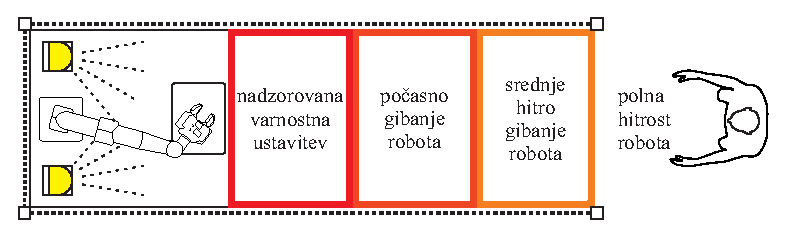
\includegraphics[width=\textwidth]{hc10_sdm.eps}
	\caption{Primer različnih področij hitrosti robota; bolj kot je področje oddaljeno, hitreje se robot lahko premika.}
	\label{fig:hc10_sdm}
\end{figure}

\subsection*{Izvedba naloge}

Pri tej nalogi boste definirali eno varnostno območje. če se bo v tem območju nahajala oseba, boste omejili gibanje robota na hitrost 50~mm/s, drugače pa se bo robot gibal s hitrostjo 250~mm/s. Za spremljanje prisotnosti človeka v varnostnem območju boste uporabili dodatni laserski skener proizvajalca SICK.

\subsubsection*{Nastavitev laserskega skenerja SICK TIM310}

V prvem delu naloge boste ustrezno sprogramili laserski skener. Pred programiranjem naprave se prepričajte, da je naprava fizično priklopljena na napajanje -- na senzorju sveti zelena LED.

Senzor priključite na računalnik preko USB kabla. Na računalniku se samodejno zažene programska oprema SOPAS, ki samodejno prepozna priključeno napravo. Za urejanje nastavitev je potrebno klikniti na ikono prepoznane naprave, ki je prikazana na sliki \ref{fig:hc10_sick1}.

\begin{figure}[!hbt]
	\centering
	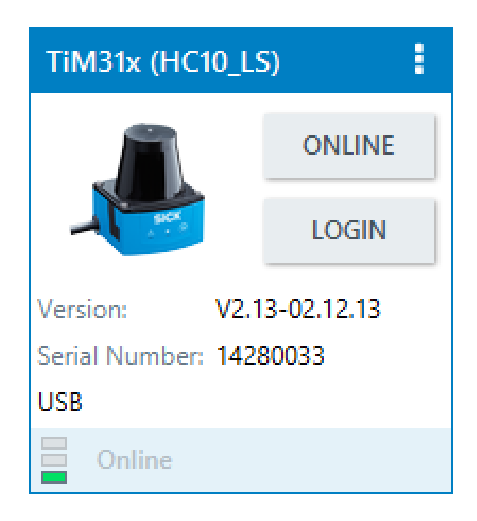
\includegraphics[width=0.3\textwidth]{hc10_sick1.eps}
	\caption{Prikaz prepoznane naprave znotraj programskega okolja SOPAS}
	\label{fig:hc10_sick1}
\end{figure}

Odpre se vam okno za urejanje nastavitev naprave, kjer se na levi strani nahaja drevesna struktura. Deli se na tri osnovne mape: \emph{Parameter}, \emph{Monitor} in \emph{Service}. Za prilagajanje delovanja senzorja je potrebno urediti nastavitve znotraj mape \textbf{Parameter} (slika \ref{fig:hc10_sick2}).

\begin{figure}[!hbt]
	\centering
	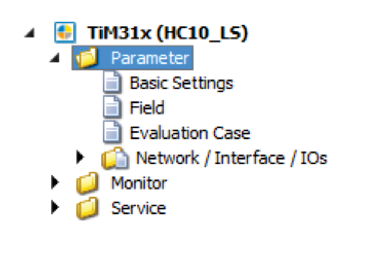
\includegraphics[width=0.3\textwidth]{hc10_sick2.eps}
	\caption{Drevesna struktura nastavitev laserskega skenerja}
	\label{fig:hc10_sick2}
\end{figure}

Najprej uredite ustrezno obliko območja znotraj katerega želimo, da senzor prepozna morebitno prisotnost. Območje naj bo po obliki in dimenziji približno enako polju, kot je prikazano na sliki \ref{fig:hc10_sick3}. Območje uredite z orodji, ki jih lahko opazimo na levi strani slike \ref{fig:hc10_sick3} (označena s številkami 1 -- 4).
\begin{itemize}
	\item Skupina orodij 1 je namenjena urejanju točk, na katerih temelji oblika polja. Prvo orodje je namenjeno dodajanju točk, drugo orodje omogoča urejanje že obstoječih točk, tretje orodje pa je namenjeno brisanju točk.
	\item Skupina orodij 2 je namenjena avtomatskemu izločanju objektov znotraj vidnega polja naprave.
	\item Skupina orodij 3 predstavlja izris prepoznanih objektov znotraj polja.
	\item Skupina orodij 4 predstavlja način prikaza polja naprave.
\end{itemize}

\begin{figure}[!hbt]
	\centering
	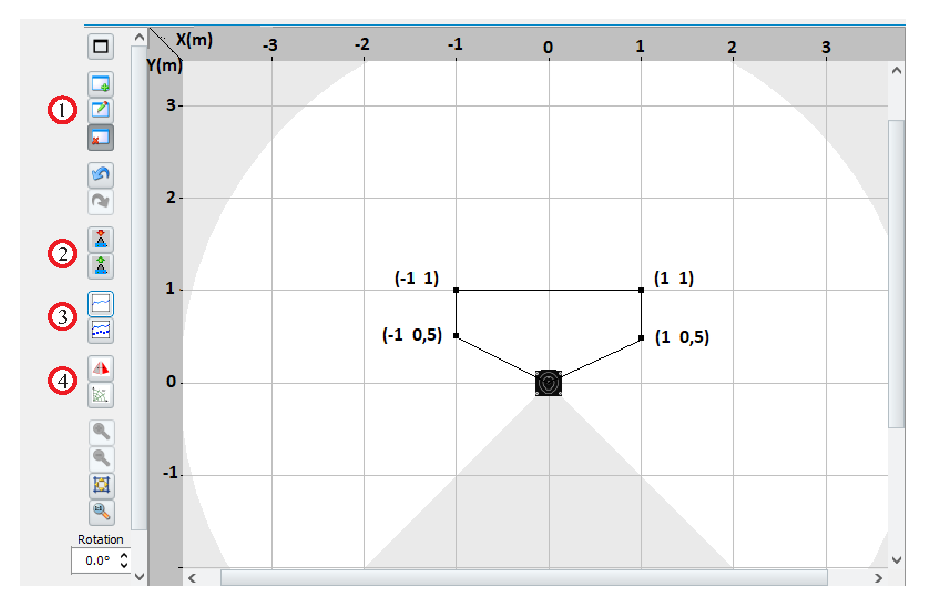
\includegraphics[width=0.9\textwidth]{hc10_sick3.eps}
	\caption{Okno za nastavljanje potrebne oblike varnostnega območja}
	\label{fig:hc10_sick3}
\end{figure}

Znotraj narisanega polja se definirajo tri varnostna območja, znotraj vsakega območja pa se spremlja morebitno prisotnost objektov. Vsako območje pro\v zi ustrezen digitalni izhod senzorja, ki je vezan naprej na FSU robotskega krmilnika. Pri vaji boste spremljali samo prisotnost osebe v srednjem območju.

Ko boste definirali ustrezno območje, definirajte tudi parametre znotraj zavihka \textbf{Evaluation Case}:
\begin{itemize}
	\item Duration time output - \v zelimo čim manjšo zakasnitev med tem, ko objekt ni več prisoten in ponovnim zagonom robota;
	\item Response time - \v zelimo, da se robot v čim krajšem času ustavi;
	\item Blanking size - \v zelimo, da senzor ne prepozna objektov manjših od 50 mm.
\end{itemize}

Z eksperimentalnim poiskušanjem poiščite ustrezne nastavitve senzorja.

Ko so vsi parametri ustrezno urejeni, zaprete okno za urejanje nastavitev naprave. Prikaže se nam opozorilo, če želimo spremembe shraniti na napravo. S tem, ko prenos potrdite, ste zaključili z nastavljanjem senzorja za prepoznavo prisotnosti. Iz senzorja izklopite USB kabel.

\subsection{Nastavitev robotskega krmilnika} \label{realni3}

V drugem delu boste ustrezno omejili hitrosti robota glede na informacijo iz laserskega skenerja. Omejitve hitrosti se nastavljajo v meniju \textbf{SAFETY FUNC.}, zavihek \textbf{SPEED LIMIT} (prikazano na sliki \ref{fig:hc10_speed1}). V tem zavihku lahko ustvarimo in nastavimo več datotek, ki omejujejo hitrost robota. Za to vajo boste ustvarili dve različni omejitvi hitrosti robota (dve datoteki): delovno hitrost ter hitrost pri interakciji (datoteka 1 in 2).

\begin{figure}[!hbt]
	\centering
	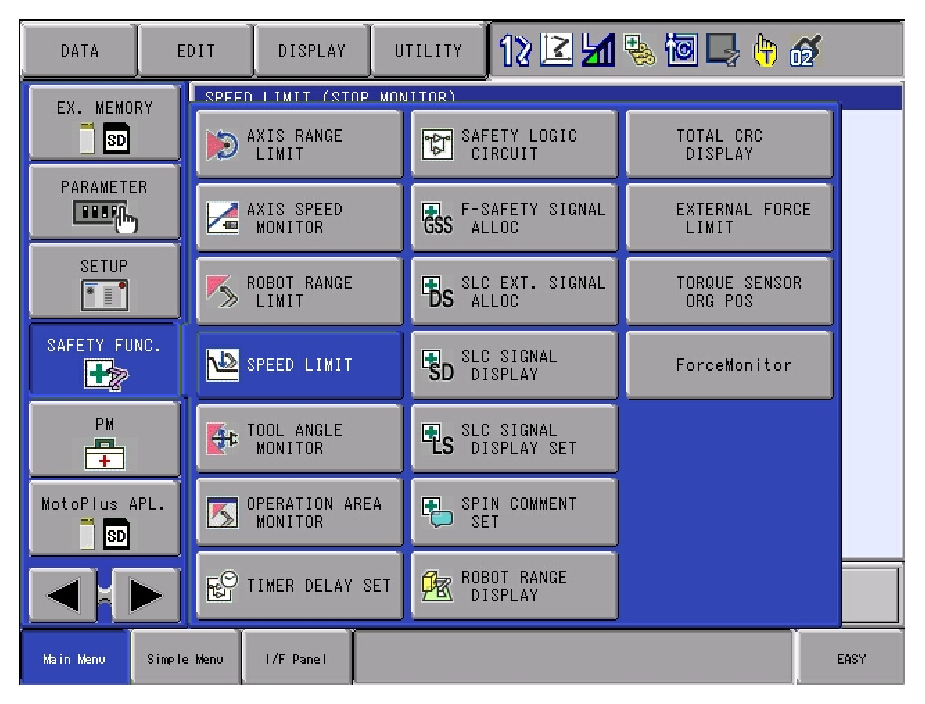
\includegraphics[width=0.7\textwidth]{hc10_speed1.eps}
	\caption{Meni Safety functions}
	\label{fig:hc10_speed1}
\end{figure}

Odpre se vam okno, ki je prikazano na sliki \ref{fig:hc10_speed2}. V tem zavihku lahko ustvarimo in nastavimo več datotek, ki omejujejo hitrost robota. Za to vajo boste ustvarili dve različni omejitvi hitrosti robota (dve datoteki): delovno hitrost ter hitrost pri interakciji (datoteka 1 in 2).

\begin{figure}[!hbt]
	\centering
	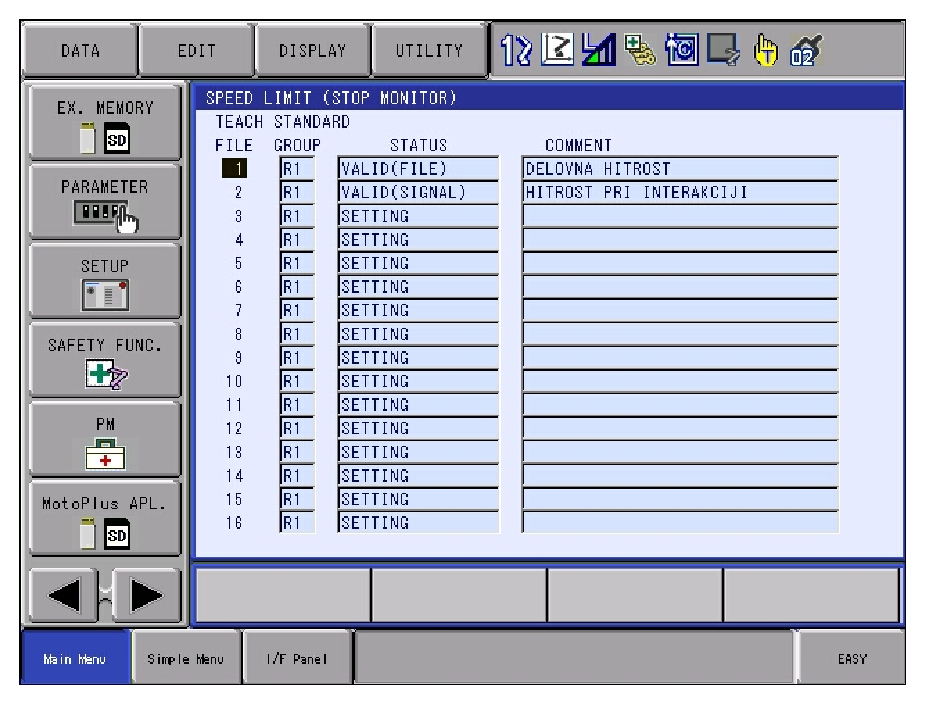
\includegraphics[width=0.7\textwidth]{hc10_speed2.eps}
	\caption{Zavihek Speed Limit}
	\label{fig:hc10_speed2}
\end{figure}

Delovno hitrost nastavite tako, da odprete prvo datoteko. S pomočjo puščic se postavimo v prvo vrstico in jo izberete s tipko \textbf{SELECT}. Odpre se vam okno, kot je prikazano na sliki \ref{fig:hc10_speed3}. V tem oknu morate ustrezno izpolniti polja \textbf{COMMENT}, \textbf{FILE VALID COND.}, \textbf{CTRL GROUP} ter \textbf{LIMIT SPEED}.

\begin{itemize}
	\item V polje \textbf{COMMENT} vpišete komentar datoteke (npr. delovna hitrost).
	\item V polju \textbf{FILE VALID COND.} nastavite, kdaj velja ta omejitev hitrosti. Lahko izbirate med \textbf{VALID}, ko omejitev velja vedno, \textbf{SIGNAL}, ko želite, da je omejitev hitrosti aktivna ob določenem pogoju (signalu), in {\textbf{INVALID}}, ko ne želite, da je omejitev aktivna. Pri tej hitrosti želite, da je omejitev vedno aktivna.
	\item V polju \textbf{CTRL GROUP} nastavite, za katerega robota velja omejitev hitrosti. V vašem primeru imate samo enega robota, zato nastavite na \textbf{R1}.
	\item V polju \textbf{LIMIT SPEED} definirate dejansko omejitev hitrosti. Za delovno hitrost nastavite omejitev na 250~mm/s.
\end{itemize}

Ostale nastavitve ostanejo nespremenjene. Nastavitve zapišete s pritiskom na gumb \textbf{READBACK} ter nato še \textbf{WRITE}. Pojavi se opozorilo, če želite posodobiti datotetko, na kar odgovorite z \textbf{YES}.

\begin{figure}[!hbt]
	\centering
	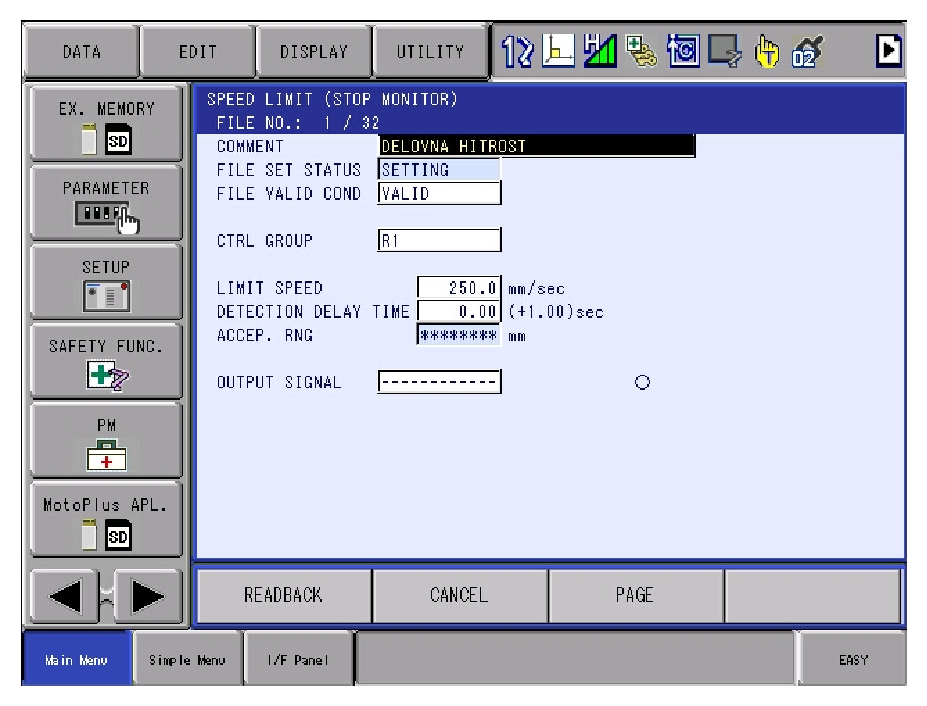
\includegraphics[width=0.7\textwidth]{hc10_speed3.eps}
	\caption{Nastavitve za delovno hitrost}
	\label{fig:hc10_speed3}
\end{figure}

Ko končate z nastavitvijo delovne hitrosti, nastavite še hitrost pri interakciji. V zavihku \textbf{SPEED LIMIT} se pomaknite na drugo vrstico in jo odprete s tipko \textbf{SELECT}. Odpre se vam okno prikazano na sliki \ref{fig:hc10_speed4}. Podobno kot pri nastavljanju delovne hitrosti moate tudi pri hitrosti interakcije ustrezno izpolniti polja \textbf{COMMENT}, \textbf{FILE VALID COND.}, \textbf{CTRL GROUP} ter \textbf{LIMIT SPEED}.

\begin{itemize}
	\item V polje \textbf{COMMENT} vpišete komentar datoteke (npr. hitrost pri interakciji).
	\item V polju \textbf{FILE VALID COND.} nastavite, kdaj velja ta omejitev hitrosti. Ta  omejitev naj bo aktivna takrat, ko laserski skener zazna osebo v svojem varnostnem območju, zato nastavite parameter na \textbf{SIGNAL}. Ob tem se vam pojavi dodatna možnost \textbf{INPUT SIGNAL}, kjer lahko definirate več pogojev oziroma signalov s poljubno logiko (\textbf{bit0} -- \textbf{bit4}). V vašem primeru gledate samo signal laserskega skenerja, ki je v robotskem krmilniku vezan na digitalni vhod  \textbf{FSBIN02( \#1)} z negativno logiko. Ta signal nastavite v polju \textbf{bit0}, kot je prikazano na sliki \ref{fig:hc10_speed4}. S parametrom \textbf{SET} nastavite negativno logiko (parameter nastavite na \emph{OFF}). Negativna logika pomeni to, da laserski skener postavi digitalni izhod na nizek nivo, ko zazna prisotnost osebe v varnostnem območju, v nasprotnem primeru pa je digitalni izhod postavljen na visok nivo. Parameter \textbf{STATUS} vam prikazuje trenutno vrednost digitalnega vhoda - poln krogec predstavlja logično 1, prazen krogec pa logično 0.
	\item V polju \textbf{CTRL GROUP} nastavite na \textbf{R1}.
	\item V polju \textbf{LIMIT SPEED} definirate dejansko omejitev hitrosti. Za hitrost ob potencialni interakciji nastavite omejitev na 50~mm/s.
\end{itemize}

Ostale nastavitve ostanejo nespremenjene. Nastavitve zapišete s pritiskom na gumb \textbf{READBACK} ter nato še \textbf{WRITE}. Pojavi se opozorilo, če želite posodbiti datotetko, na kar odgovorite z \textbf{YES}.

\begin{figure}[!hbt]
	\centering
	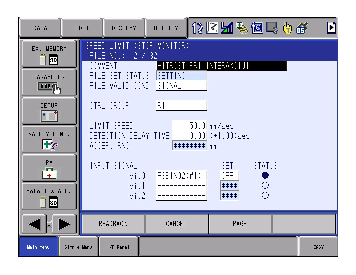
\includegraphics[width=0.7\textwidth]{hc10_speed4.eps}
	\caption{Nastavitve za hitrost pri interakciji}
	\label{fig:hc10_speed4}
\end{figure}

\subsection{Testiranje omejevanja hitrosti} \label{test3del}

Za testiranje funkcionalnosti omejevanja hitrosti izberite vaš program, ki ste ga napisali v II. delu. Poženite ga v \textbf{RUN} načinu: postavite se na začetek programa, ključ na učni enoti postavite na srednjo pozicijo, prižgite motorje s \textbf{SERVO ON READY} in pritisnete zeleni gumb na vrhu učne enote.

Za testiranje se odmaknite iz vidnega polja senzorja. Robot se mora premikati s hitrostjo 250~mm/s. Ko nekdo vstopi v varnostno območje senzorja, se mora hitrost robota opazno zmanjšati na 50~mm/s.

Na podoben način bi lahko definirali še omejitve hitrosti za ostali dve območji. Pri tem bi območje najbližje robotu (najbolj nevarno zaradi največje možnosti trka) zahtevalo vklop varnostno nadzorovane ustavitve.



